%!TeX program = xelatex
\documentclass[12pt,hyperref,a4paper,UTF8]{ctexart}
\usepackage{SJTUReport}

%%-------------------------------正文开始---------------------------%%
\begin{document}

%%-----------------------封面--------------------%%
\cover

%%------------------摘要-------------%%
%\begin{abstract}
%
%在此填写摘要内容
%
%\end{abstract}

\thispagestyle{empty} % 首页不显示页码

%%--------------------------目录页------------------------%%
\newpage
\tableofcontents

%%------------------------正文页从这里开始-------------------%
\newpage

%%可选择这里也放一个标题
%\begin{center}
%    \title{ \Huge \textbf{{标题}}}
%\end{center}

\section{实验目的}
\begin{itemize}
    \item 掌握凝聚法制备$Fe(OH)_3$胶体分散体系及其纯化方法。
    \item 观察溶胶的电泳现象并了解其电学性质。
    \item 掌握电泳法测定胶粒电泳速率的技术,计算胶粒$\xi$电势。
\end{itemize}

\section{实验原理}
胶体分散相粒子的尺度一般在$10^{-9}$-$10^{-7}m$之间,因此胶体的制备原则上可由分子或离子凝聚成胶粒,或由大块物质分散成胶粒。前一种制备方法称为凝聚法,后一种方法称为分散法。分散相在分散介质中的溶解度微小是形成增液溶胶的必要条件之一。只有分散相的溶解度微小,在分散法中形成的小粒子才不至于因溶解而消失。在凝聚法中还要求反应物浓度较稀,使生成的难溶物晶粒很小且没有机会长大,这样才能得到所需尺度的胶粒。如果反应体系的反应物浓度很大,则可在瞬间生成大量细小的难溶物晶粒,但是由于所形成晶粒的浓度高,相互距离近,胶粒间有可能联结在一起,故最终可能形成半透明半固体状的凝胶。

凝聚法可分为化学凝聚法和物理凝聚法两大类。若化学反应生成难溶性化合物,则在一定条件下,就能将此化合物制成胶体溶液。首先让反应在稀溶液中进行,其目的是使晶粒的增长速度放慢,保证能制备$10^{-9}$-$10^{-7}m$尺度的粒子,使体系的沉降稳定性得到保证;其次是让一种反应物过量,其目的是在晶体表面形成扩散双电层-聚集稳定性的基本因素。

由于本身的电离或选择性地吸附一定量的离子以及其他原因所致,胶粒表面带有一定量的电荷,胶粒周围的介质中分布着反离子。反离子所带电荷与胶粒表面电荷符号相反、数量相等,整个溶胶体系保持电中性。胶粒周围的反离子由于静电引力和热扩散运动的结果形成了两部分---紧密层和扩散层。紧密层约有一两个分子层厚,紧密吸附在胶核表面上,而扩散层的厚度则随外界条件(温度,体系中电解质浓度及离子的价态等)而改变,扩散层中的反离子符合玻耳兹曼(Boltzmann)分布。由于离子的溶剂化作用,紧密层结合有一定数量的溶剂分子,在电场的作用下,它和胶粒作为一个整体移动,而扩散层中的反离子则向相反的电极方向移动。这种在电场作用下分散相粒子相对于分散介质的定向迁移称为电泳。

研究电泳的方法主要分为界面移动电泳、区域电泳和显微电泳。本实验用界面移动电泳方法。界面移动电泳是将有色溶胶置于下图所示的界面移动电泳仪中,直接用肉眼观察溶胶界面的移动。在实验时间t内界面移动的距离为x,则胶粒的电泳速率
\begin{equation}
    u = \frac{x}{t}
\end{equation}

胶粒的运动实际上是切动面(滑动面)相对于分散介质的运动,$\xi$电势反映了胶粒表面带电荷的情况,因此$\xi$电势是一个重要的物理量。从原则上讲,胶体体系的任何一种电动现象都可用来测定和求算$\xi$电势,最方便常用的是用电泳或电渗速率求$\xi$电势。电泳或电渗的速率可通过实验测定。由于外加电解质对电泳和电渗速率有影响,因此测定电泳或电渗的速率也可用于研究外加电解质对$\xi$电势的影响。

对于非导电性胶粒的研究表明,$\xi$电势可表示为
\begin{equation}
    \xi = \frac{K\pi \eta u}{4\varepsilon_r \varepsilon_0 E}
\end{equation}

式中:$\eta$为溶液的黏度,u为电泳或电渗速率,E为电势梯度,$\varepsilon_r$为分散介质的相对介电常数,是分散介质的介电常数与真空介电常数($\varepsilon_0 = 8.854\times 10^{-12}C^2 \cdot N^{-1} \cdot m^{-2}$)之比,K为与粒子形状有关的量,1/K具有长度单位,称为双电层参照厚度。若对球形胶粒进行实验,则式(2)可变形为:
\begin{equation}
    \xi = \frac{3\eta u}{2\varepsilon_r \varepsilon_0 E}
\end{equation}

(3)式称为休格尔(Huckel)公式。若为电渗实验或棒状胶粒进行电泳实验,则(3)式可变形为
\begin{equation}
    \xi = \frac{\eta u}{\varepsilon_r \varepsilon_0 E}
\end{equation}

(4)式称为Helmholz-Smoluchowski公式。

当辅助液的电导率和所测溶胶的电导率接近时,两电极间的电势梯度E可近似表示为
\begin{equation}
    E = \frac{U}{l}
\end{equation}

式中的U为加在两电极间的电势降,l为两电极间的距离。

实验证明电泳实验测得胶粒的电迁移率约为$2-4\times 10^{-8} m^2\cdot s^{-1} \cdot V^{-1}$,这与普通离子的迁移率非常相近。由于胶粒的质量是普通离子的几千倍,故可证明胶粒不仅带电荷,而且所带电荷量相当大。胶粒的制备条件,粒子的大小,形状以及表面带电荷量,溶液中电解质的种类,浓度,介质的pH,温度以及所加的电压等均会影响胶粒的电泳速率。蛋白质在pH比等电点大或小的介质中也带不同种类的电荷。

\begin{figure}[htp]
    \centering
    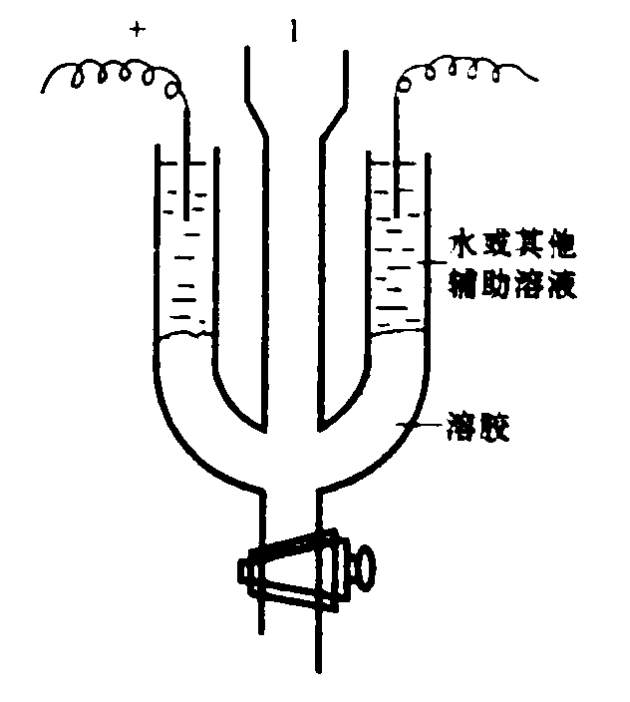
\includegraphics[width=0.3\linewidth]{截屏2023-12-11 23.03.00.png}
    \caption{界面移动电泳仪示意图}
    \label{fig:enter-label1}
\end{figure}



\section{仪器与试剂}
\subsection{实验仪器}
\begin{itemize}
    \item DYY-1C稳压电泳仪1套
    \item 电导率仪1台
    \item 电泳管1支
\end{itemize}


\subsection{实验试剂}
\begin{itemize}
    \item 无水$FeCl_3$(A.R.)
    \item 0.1$mol\cdot dm^{-3}$KCl
    \item 高分子半透膜袋(相对摩尔质量$3\times 10^4$以下可通过)
\end{itemize}


\section{实验步骤}
\subsection{$Fe(OH)_3$溶胶的制备}
    
    \begin{itemize}
        \item 在托盘天平上称取0.5g无水$FeCl_3$于50mL烧杯中,加入20mL去离子水溶解。
        \item  在500mL烧杯中加入200mL去离子水煮沸,在搅拌下滴加$FeCl_3$溶液,控制时间约5min加完。水浴保温。
    \end{itemize}

\subsection{$Fe(OH)_3$溶胶纯化}
 \begin{itemize}
 	\item     将冷却至室温的$Fe(OH)_3$溶胶转移到半透膜袋中,扎紧袋口,将半透膜袋放入1000mL烧杯中,加入去离子水至半透膜袋完全浸入,进行渗析,除去电解质。每10min换一次去离子水,共渗析4-5次,渗析过程中应经常搅拌半透膜袋外面的去离子水以提高渗析效率
 \end{itemize}   

\subsection{$Fe(OH)_3$溶胶电泳速率测定}

    \begin{itemize}
        \item 将$0.1mol\cdot dm^{-3}$HCl溶液用去离子水调节至电导率与经纯化的$Fe(OH)_3$溶胶相同作为辅助液。先使用少量辅助液润洗电泳仪大活塞下部部分,润洗完成后将辅助液注入中间管至液面高于电泳仪大活塞。

        \item 关闭大活塞,打开小活塞,使用$Fe(OH)_3$溶胶仔细润洗电泳仪大活塞上部部分,润洗结束后将$Fe(OH)_3$溶胶沿管壁缓慢加入,至液面高于电泳仪顶部连通管为止。插入铂电极,缓慢打开大活塞,防止$Fe(OH)_3$溶胶与辅助液界面相混影响肉眼对于电泳迁移界面的判断。

        \item 连接电路,接通电源,将电泳仪的电压档调节至80V,观察溶胶液面与辅助液界面的相对移动速率与方向,记下界面迁移约1cm时所耗的时间,停止实验,用线测量出两电极间的距离。

    \end{itemize}
\section{数据记录}
\subsection{数据整理}
\begin{table}[h]
	\centering
	\begin{tabular}{|c|c|c|}
		\hline
		变量 & 值 & 单位 \\
		\hline
		x & 1 & cm \\
		\hline
		t & 1072 & s \\
		\hline
		l & 52 & cm \\
		\hline
		U & 80 & V \\
		\hline
		实验温度 & 25 & $^{\circ}C$ \\
		\hline
	\end{tabular}
	\caption{实验数据记录表}
\end{table}


\subsection{实验记录}
\begin{figure}[htp]
	\centering
	\begin{minipage}{0.45\linewidth}
		\centering
		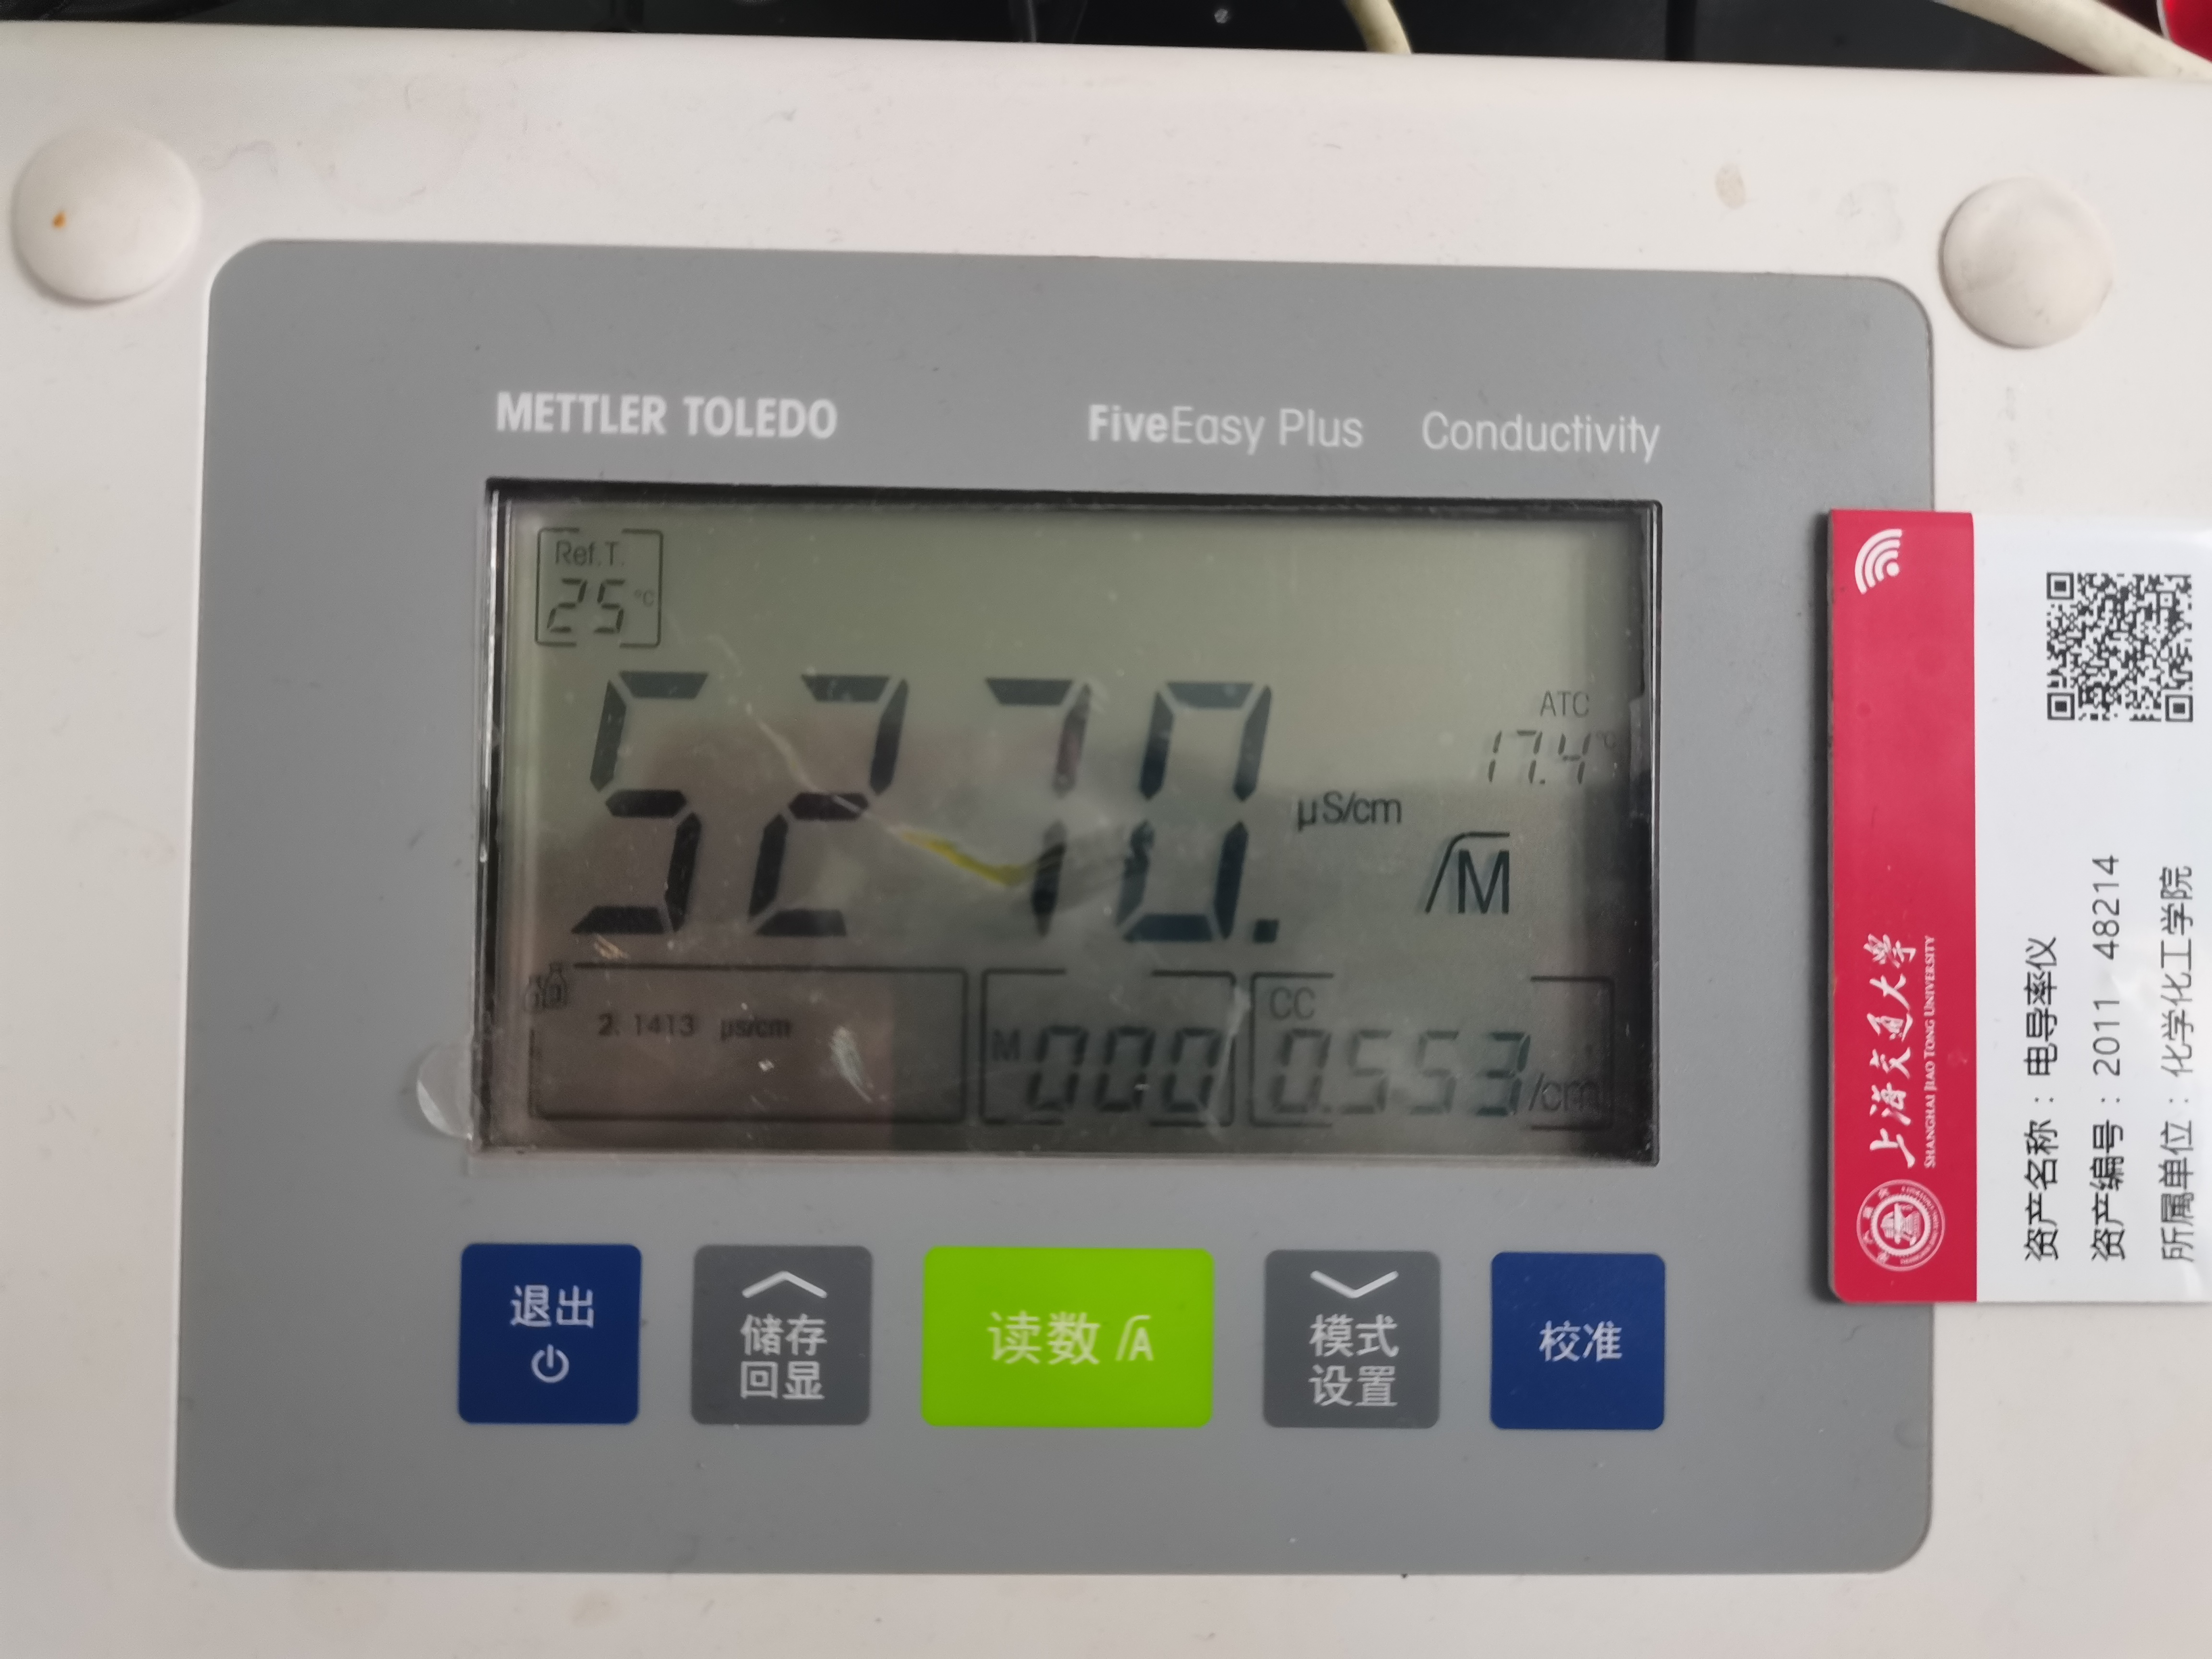
\includegraphics[width=\linewidth]{WechatIMG604.jpg}
		\caption{$Fe(OH)_3$溶胶电导率}
		\label{fig:gel-conductivity}
	\end{minipage}\hfill
	\begin{minipage}{0.45\linewidth}
		\centering
		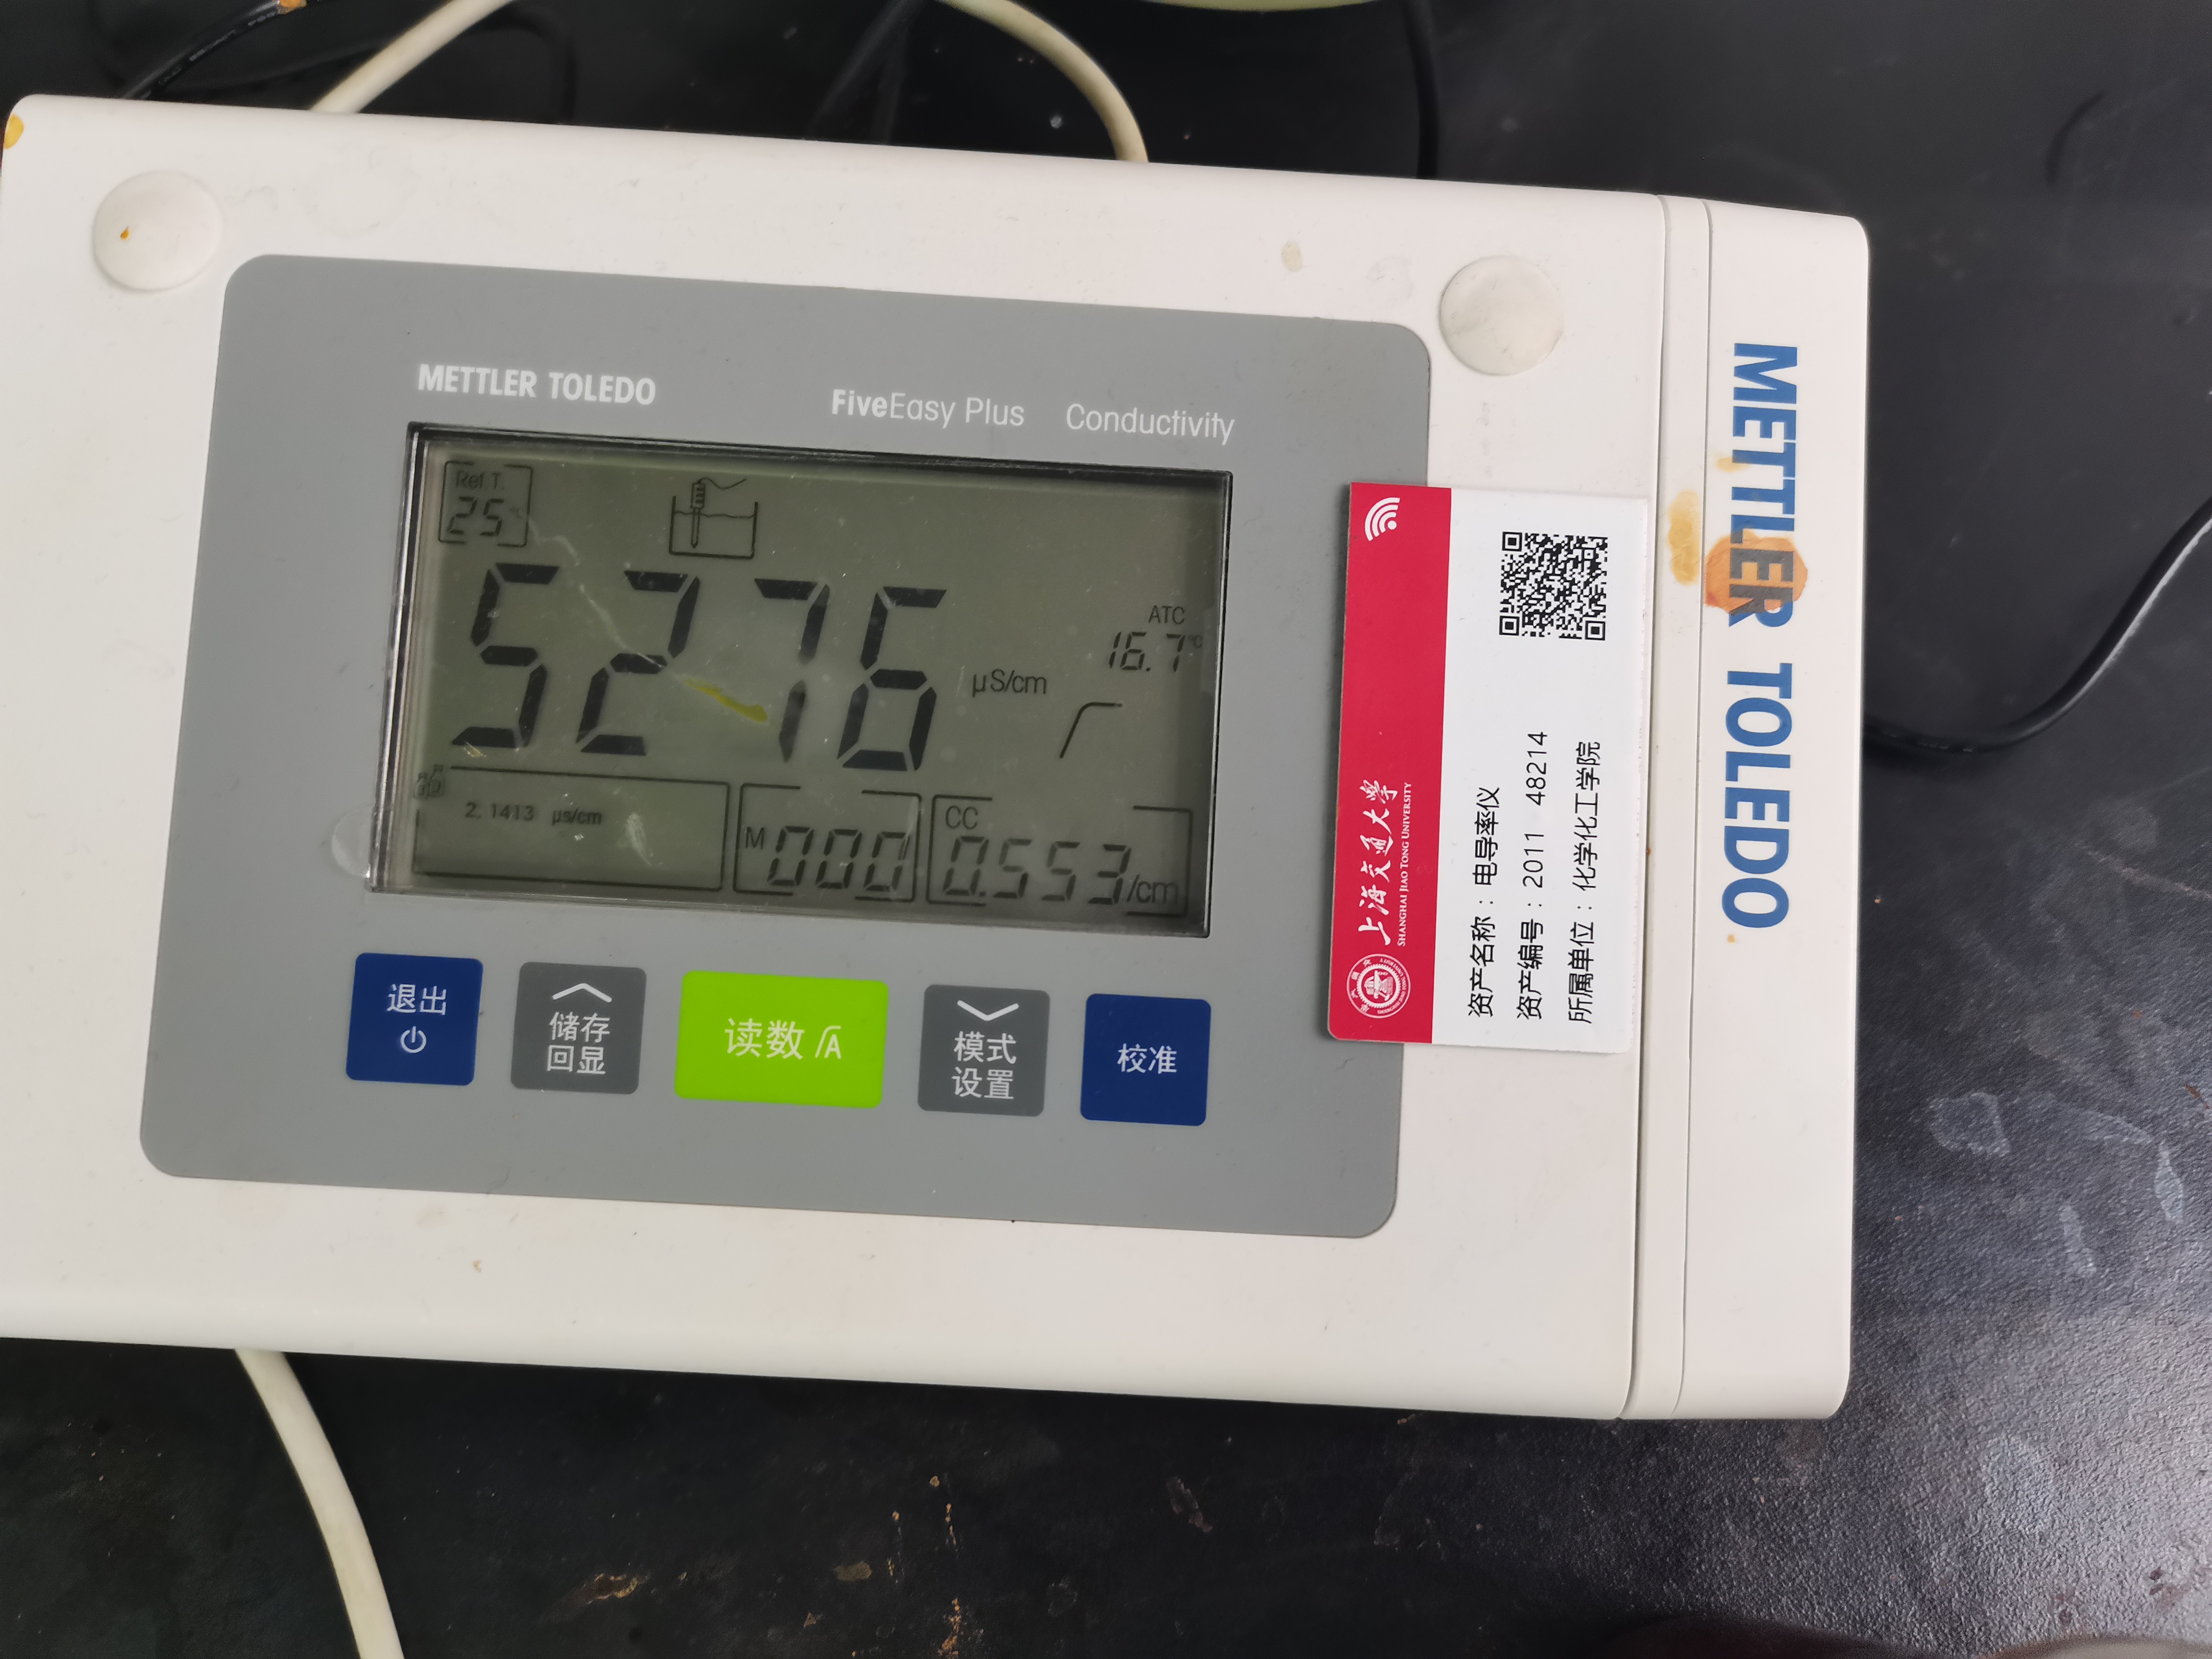
\includegraphics[width=\linewidth]{WechatIMG605.jpg}
		\caption{HCl溶液调节后电导率}
		\label{fig:hcl-conductivity}
	\end{minipage}
\end{figure}
\newpage

\section{数据处理和分析}

在电泳实验中,胶粒的迁移速率(u)是通过测量迁移距离(x)与迁移时间(t)得到的。迁移速率可以用下式计算:

\begin{equation}
	u = \frac{x}{t} = \frac{0.01 \text{ m}}{1072 \text{ s}} = 9.328 \times 10^{-6} \text{ m s}^{-1}
\end{equation}

实验中,电极间的电势梯度(E)是通过测量电极间距离(l)和电势降(U)得到的,计算公式如下:

\begin{equation}
	E = \frac{U}{l} = \frac{80 \text{ V}}{0.52 \text{ m}} = 153.85 \text{ V m}^{-1}
\end{equation}

在室温($25^{\circ}C$)下,水的黏度和相对介电常数是确定的。根据文献资料,水的黏度在$25^{\circ}C$时约为$0.89 \times 10^{-3} \text{Pa·s}$\cite{1},而相对介电常数在同温度下约为78.4\cite{2}。因此,可以根据以下公式估算电泳速率对应的电势($\varepsilon$):

对于假设为球形的胶粒,电势由以下公式给出:

\begin{equation}
	\varepsilon_{\text{球形}} = \frac{3 \eta_{25^{\circ}C} u}{2 \varepsilon_r \varepsilon_0 E} = 103.64 \text{ mV}
\end{equation}

对于假设为棒状的胶粒,电势由以下公式给出:

\begin{equation}
	\varepsilon_{\text{棒状}} = \frac{\eta_{25^{\circ}C} u}{\varepsilon_r \varepsilon_0 E} = 69.10 \text{ mV}
\end{equation}

在本实验中,观察到$Fe(OH)_3$溶胶界面朝向阴极移动,表明胶粒带有正电荷。

\section{结果讨论与分析}
\subsection{误差分析与实验反思}
本实验测得$Fe(OH)_3$胶体双电层电位为103.64mV(球形),69.10mV(棒状)。由于氢氧化铁胶体的双电层点位并不存在一个固定的值,它瘦很多因素影响,故没有一个标准值用于分析误差;但根据文献《氢氧化铁胶体制备与性质实验的改进》\cite{3}中胶体双电层电位$\varepsilon$测定值约在40mV左右浮动综合上述成果,推断得到本实验测定结果偏大。可能的实验误差如下:
\begin{enumerate}
    \item 测量电泳仪中两电极间的距离时,所采用的绳线测量法难以保证绳线在电泳仪内部保持绝对的紧绷状态,因此所得的电极间距离测量带有估计成分,增加了误差。由于氢氧化铁胶体的双电层电位的计算公式中,电极间距离对最终结果具有显著的影响,这种测量误差可能导致最终双电层电位的计算结果偏离真实值。
    \item 在本次实验中,氢氧化铁胶体与辅助电解液之间的界面因为大活塞的过度操作而受到了显著扰动,导致界面边界的模糊,对界面位移的观测造成了难以精确判断的状况。这种模糊不清的界面导致了在胶粒电泳速率测定中界面移动距离x与理论值之间的偏差,影响了最终的电泳速率的精确度。
    \item 在渗析过程中,为了提高渗析效率通常需要对半透膜外部的去离子水进行持续搅拌,以促进溶质的扩散和浓度梯度的维持。然而,在具体的实验操作中,由于烧杯尺寸的限制,可能未能进行充分的搅拌,这会导致渗析效率降低,影响渗析的完整性和均匀性,从而对实验结果产生负面影响。
    \item 在溶胶制备过程中,采用的是将氯化铁溶液滴加到沸腾的去离子水中,并伴随搅拌,这一步骤旨在促进铁离子的充分水解。理想情况下,滴加完成后应在水浴中保持一定时间的保温,确保$Fe^{3+}$ 离子能够完全水解形成氢氧化铁胶体。若实验中未执行这一保温步骤,加之搅拌效果受限,就可能导致水解反应不充分,从而影响氢氧化铁胶体的质量和均匀性。
    \item 胶体制备时水解时间应该控制在煮沸 5min 左右。时间太短 $Fe^{3+}$不能完全水解,时间过长 $Fe(OH)_3$溶胶粒子会不断聚集长大
    \item 据文献《氢氧化铁溶胶制备条件对其电泳等性能的影响》\cite{4}所述,铁氯化物($FeCl_3$)的浓度对氢氧化铁($Fe(OH)_3$)溶胶的双电层电位($\varepsilon$)及其稳定性有显著影响。在水解过程中,使用较高浓度的$FeCl_3$会导致生成的氢氧化铁胶粒粒径增大,从而使溶胶体系的稳定性降低。在本实验中,所使用的$FeCl_3$溶液浓度为$0.014mol\cdot dm^{-3}$,而根据相关研究,配制成浓度为$0.010mol\cdot dm^{-3}$的$FeCl_3$溶液时,测量所得的电泳等性能表现更为理想。
\end{enumerate}

对于误差的分析,下面也列举出了相应的改进方法。首先,对于电极间距离的测量,应该采用更为精密的测量工具,确保距离数据的精确性,从而有效减小双电层电位计算中的误差。在操作过程中,特别是在形成氢氧化铁胶体与辅助电解液界面时,必须尽可能地减少操作带来的扰动,这要求在移动大活塞时更为谨慎和精确,以保障界面的清晰度和测量的准确性。此外,对于渗析过程中的搅拌,应保证其均匀性和连续性,这可能需要使用更适宜的搅拌设备和更大体积的容器以提升渗析效率。在溶胶制备阶段,应标准化水解条件,控制滴加速率和保温时间,确保铁离子的完全水解,以改善氢氧化铁胶体的质量。最后,详细考量文献中推荐的化学试剂浓度,精确配制$FeCl_3$溶液的浓度,例如降低至$0.010mol\cdot dm^{-3}$,有助于提高溶胶的稳定性并获得更加精准的电位测量结果。通过这些细致的实验设计和操作上的考量,可以极大地提升实验数据的可靠性,为科学研究的精确性和复现性提供坚实的基础。


\subsection{实验总结}
在本次实验中,我们成功地通过凝结法制备了$Fe(OH)_3$胶体分散体系,并对其进行了纯化处理。实验不仅让我们观察到溶胶的电泳现象,而且还加深了我们对胶体电学性质的理解。通过使用电泳法,我们测定了胶粒的电泳速率,并进一步计算出了胶粒的ξ电势,这对理解胶体颗粒的表面电荷情况至关重要。实验过程中,我们首先学习了胶体的制备原理,包括分散相粒子的尺度和凝聚法的应用。我们了解到,在凝聚法中,控制反应物浓度可以有效地制备所需尺度的胶粒,而过量的反应物则有利于在晶体表面形成扩散双电层,从而提供聚集稳定性。随后,实验指导我们进行了$Fe(OH)_3$溶胶的制备与纯化,并测量了其电泳速率。通过实验,我们观察到胶粒在电场中的迁移现象,也对胶粒表面的电荷分布有了直观的理解。数据处理和分析阶段,我们采用公式计算了胶粒的$\varepsilon$电势,并对实验数据进行了仔细的整理。通过比较不同条件下胶粒的电泳速率,我们还研究了外加电解质对$\varepsilon$电势的影响。

总的来说,本次实验不仅提升了我们对胶体科学的理论知识,同时也锻炼了我们的实验操作技能和数据分析能力。在结果讨论与分析部分,我们对实验中可能出现的误差进行了分析,并提出了改进措施。

\section{思考题}
\subsection{从实验中你是如何体会“胶体是物质存在的一种状态,而不是一种特殊物质”这句话的?}

    胶体是一种复杂的物质系统,其特征在于其中的微观颗粒(被称为胶粒)悬浮在另一种物质中,形成一个均匀分散的体系。整个胶体往往分为胶粒与扩散层,由于离子的溶剂化作用,胶粒中的吸附层结合有一定数量的溶剂分子,在电场的作用下,它和胶粒核心作为一个整体移动,而扩散层中的反离子则向相反的电极方向移动。因此,在本实验使用电泳的过程中,胶粒与扩散层往相反方向移动,可以通过观察胶体中的微粒子在电场中的运动情况,确定微粒子的电荷性质。同时,还可以通过调节胶体系统的条件,如pH值与温度,改变胶体中的电荷分布情况,从而影响电泳运动。因此有上述现象可得,胶体并不是完整而稳定的一种物质,而是物质存在的一种相对松散的状态,外界条件的变化能够较为容易地改变其状态。
\subsection{$Fe(OH)_3$溶胶胶粒总是带负电荷吗?}
氢氧化铁($\text{Fe(OH)}_3$)溶胶中胶粒的电荷状态并非恒定,而是受溶液pH值及其他环境因素的影响。在中性或碱性环境下,$\text{Fe(OH)}_3$胶粒倾向于携带负电荷,这是由于在这种pH条件下,氢氧化铁表面促使羟基离子($\text{OH}^-$)的吸附,从而在胶粒表面形成负电荷。相反,在酸性条件下,胶粒表面可能会吸附质子($\text{H}^+$),结果导致胶粒表面带正电荷。溶液的离子强度和其他离子种类的存在也可能对$\text{Fe(OH)}_3$溶胶胶粒的电荷状态产生显著影响。例如,特定盐类的添加可导致表面电荷性质的改变。因此,$\text{Fe(OH)}_3$溶胶胶粒的电荷特性并非固定不变,而是一个受特定化学环境影响的动态特性。
\subsection{胶粒的胶核由m个分子组成,对同一种胶体粒子m是否为定值?}


    不是,对于胶体粒子,"m" 表示胶粒的胶核由多少个分子构成。对于同一种胶体粒子,这个数字可能不是一个严格固定的值,因为胶体粒子的大小和形状可能会在一定范围内有所不同。在自然条件下,胶体粒子的大小分布通常是多种多样的。
\subsection{写出本实验中$Fe(OH)_3$溶剂胶团结构}

    ${\{ [Fe(OH)_3]_m \cdot nFeO^{+} \cdot (n-x)Cl^{-} \} }^{x+} \cdot xCl^{-}$

    其中$[Fe(OH)_3]_m$为胶核,$nFeO^{+}$为电位离子,与反离子$(n-x)Cl^{-}$构成吸附层,进而与胶核构成胶粒。反离子$xCl^{-}$为扩散层。

\begin{align}
	\text{FeCl}_3 + 3\text{H}_2\text{O} &\rightarrow \text{Fe(OH)}_3 + 3\text{HCl} \\
	\text{Fe(OH)}_3 + 3\text{HCl} &\rightarrow \text{FeOCl} + 2\text{H}_2\text{O} \\
	\text{FeOCl} &\rightarrow \text{FeO}^+ + \text{Cl}^-
\end{align}

由于初始加入的氯化铁浓度较低,因此形成的$\text{Fe(OH)}_3$以胶体形式存在而非沉淀。氢氧化铁胶体粒子与盐酸反应生成氯氧化铁($\text{FeOCl}$),随后电离为铁氧正离子($\text{FeO}^+$)与氯离子($\text{Cl}^-$)。由于铁氧正离子与氢氧化铁($\text{Fe(OH)}_3$)胶粒具有相同的金属离子(铁),氢氧化铁胶粒将吸附$\text{FeO}^+$,而氯离子的共同作用下,形成了胶体粒子。

\subsection{电泳速率与哪些因素有关?}
电泳速度的快慢与溶胶的电势、介质的介电常数$\varepsilon$、电泳仪两级间的电位差 U 成正比,与溶胶的黏度、电泳仪两级间的距离成反比。




\reference

\end{document}